\documentclass[smaller]{beamer}

\usepackage{helvet}
\usepackage{hyperref, graphicx}
\usepackage{amsthm}
\usepackage{amsfonts}
\usepackage{etoolbox}
\usepackage{wrapfig}
\usepackage{tikz}
\usepackage{ulem}
\usepackage{fontspec}
%\usepackage[T1]{fontenc}
%\setmainfont{Cambria}
%\usefonttheme{serif}

\usetheme{default}
\setbeamertemplate{navigation symbols}{}
\AtBeginSection[ ]
{
\begin{frame}{Outline}
    \tableofcontents[currentsection]
\end{frame}
}

% Default fixed font does not support bold face
\DeclareFixedFont{\ttb}{T1}{txtt}{bx}{n}{11} % for bold
\DeclareFixedFont{\ttm}{T1}{txtt}{m}{n}{12}  % for normal - use in headings

% Custom colors
\usepackage{color}
\definecolor{TUGray}{RGB}{101,101,137}
\definecolor{TUBlack}{RGB}{30,0,0}
\definecolor{mygreen}{RGB}{45,111,63}
\definecolor{keywords}{RGB}{205,114,0}
\definecolor{comments}{RGB}{181,51,139}
\definecolor{strings}{RGB}{58,144,81}
\definecolor{numeric}{RGB}{66,110,176}
\definecolor{linos}{rgb}{0.4,0.4,0.4}
\definecolor{links}{rgb}{0,0.4,0.75}

\definecolor{bggray}{RGB}{232, 233, 235}

\usecolortheme[named=mygreen]{structure}
\setbeamercolor{normal text}{fg=TUBlack}\usebeamercolor*{normal text}

\setbeamercolor{codecol}{fg=TUGray!25!black,bg=bggray}

\hypersetup{colorlinks, linkcolor=links, urlcolor=links}



\usepackage[sfdefault,scaled=.85]{FiraSans}
\usepackage{newtxsf}

\usepackage{listings}

\newtoggle{InString}{}% Keep track of if we are within a string
\togglefalse{InString}% Assume not initally in string

\newcommand\digitstyle{\color{numeric}}
\makeatletter
\newcommand{\ProcessDigit}[1]
{%
  \ifnum\lst@mode=\lst@Pmode\relax%
   {\digitstyle #1}%
  \else
    #1%
  \fi
}
\makeatother

\lstset{literate=%
    {0}{{{\ProcessDigit{0}}}}1
    {1}{{{\ProcessDigit{1}}}}1
    {2}{{{\ProcessDigit{2}}}}1
    {3}{{{\ProcessDigit{3}}}}1
    {4}{{{\ProcessDigit{4}}}}1
    {5}{{{\ProcessDigit{5}}}}1
    {6}{{{\ProcessDigit{6}}}}1
    {7}{{{\ProcessDigit{7}}}}1
    {8}{{{\ProcessDigit{8}}}}1
    {9}{{{\ProcessDigit{9}}}}1
	{<=}{{\(\leq\)}}1
	{>=}{{\(\geq\)}}1,
	% morestring=[b]",
    % morestring=[b]',
    % morecomment=[l]{//},
}

\lstdefinelanguage{Pseudo}{
    morekeywords={return, while, if, else, for, input},
    morecomment=[l]{\#},
}

% Pseudocode style
\newcommand\pseudostyle{\lstset{
language=Pseudo,
basicstyle=\fontfamily{ccr}\scriptsize,
commentstyle=\it\scriptsize\color{linos},
keywordstyle=\it\bfseries\scriptsize,
mathescape=true,
literate=
    {=}{$\leftarrow{}$}{1}
    {==}{$={}$}{1}
    {<=}{{\(\leq\)}}1
	{>=}{{\(\geq\)}}1,
xleftmargin=18pt,
xrightmargin=4pt,
aboveskip=12pt,
belowskip=0pt,
frame=tB,
keepspaces=true
}}

% Python style for highlighting
\newcommand\pythonstyle{\lstset{
language=Python,
basicstyle=\ttfamily\tiny,
numbers=left,
numberstyle=\tiny\color{linos},
morekeywords={self, np},              % Add keywords here
keywordstyle=\tiny\color{keywords},
commentstyle=\it\tiny\color{comments},    % Custom highlighting style
stringstyle=\tiny\color{strings},
xleftmargin=18pt,
xrightmargin=4pt,
aboveskip=0pt,
belowskip=0pt,
escapeinside={(*@}{@*)},
frame=l,                         % Any extra options here
showstringspaces=false,
keepspaces=true
}}

% Pseudocode environment
\lstnewenvironment{pseudo}[1][]
{
    \pseudostyle
    \lstset{
        #1
    }
}
{}

% Python environment 
\lstnewenvironment{python}[1][]
{
	\pythonstyle
	\lstset{
	#1
	}
}
{}

% wrap the Python environment
\newenvironment{codeblock}
    {\hfill\begin{beamerboxesrounded}[lower=codecol, width=0.8\textwidth]
    \medskip

    }
    { 
    \end{beamerboxesrounded}\hfill
    }

\theoremstyle{example}
\newtheorem{question}{Question}

\newcommand{\ct}[1]{\lstinline[language=Python]!#1!}
\newcommand{\ttt}[1]{{\small\texttt{#1}}}
\newcommand{\lsitem}[2]{\ttt{{#1}[}\ct{#2}\ttt{]}}

\newcommand{\x}{\textbf{x}}
\newcommand{\ix}[1]{{\it #1}}

\author{Chris Cornwell}
\date{April 1, 2025}
\title{A survey of some Machine Learning models}

\begin{document}

\begin{frame}
\titlepage
\end{frame}

\section{Support Vector Machines, continued}

%%%%
\begin{frame}
\frametitle{Review - Goal of Maximum margin}
    The goal with a support vector machine, given sample data $\{(\x_i, \ix y_i)\}_{i=1}^n$, with $\x_i\in\mathbb R^d$, is to find parameters $\omega=(\textbf{w},b)$, where $\textbf{w}\in\mathbb R^d$ and $b\in\mathbb R$, so that $\ix y_i(\textbf{w}\cdot{\x}_i + b) \ge 1$ is satisfied for all $i$, and the norm of $\textbf{w}$ is minimized (conventionally, you use half of the norm squared as a function to minimize).
    
    \pause
    Minimizing the norm of $\textbf{w}$ makes the \textit{marginal hyperplanes}, where $\textbf{w}\cdot{\x} + b = \pm 1$, be as far as possible from the hyperplane $\{\x\ |\ \textbf{w}\cdot\x + b = 0\}$ as possible.

    \centering
    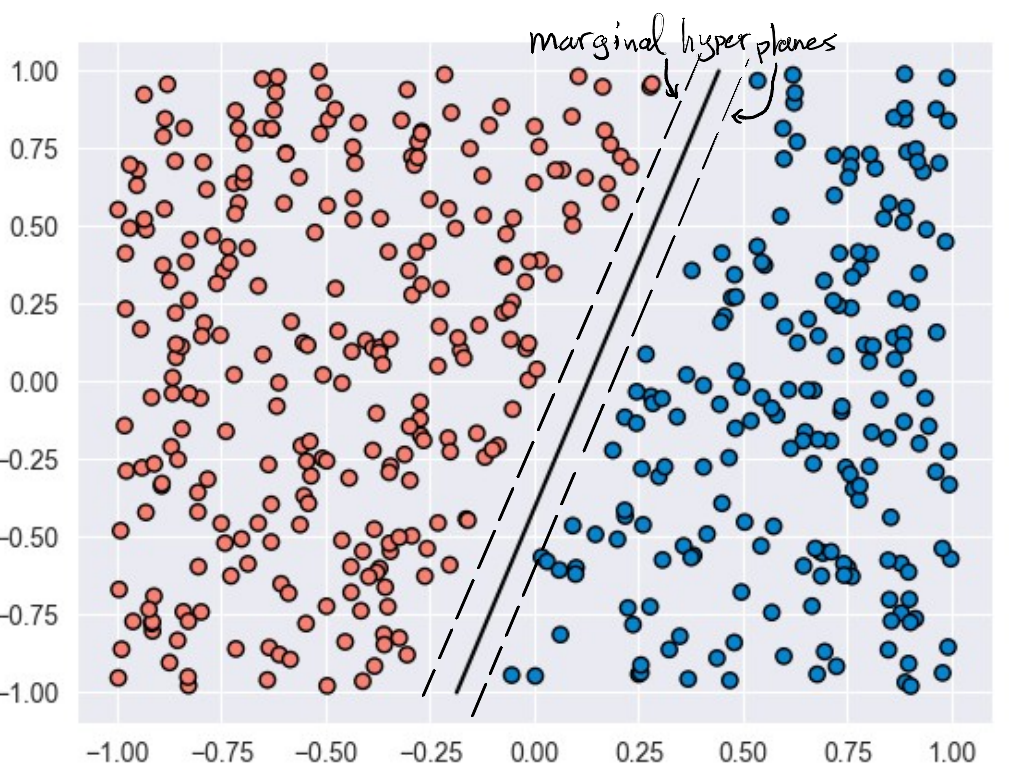
\includegraphics[height=0.35\textheight]{../../Images/Hfit-simulated-marginal-hyperplanes.png}
\vspace*{12pt}

\end{frame}

%%%%
\begin{frame}
\frametitle{Using the method of Lagrange multipliers}
Recall, can understand minimizing $\frac12|\textbf{w}|^2$ subject to $\ix y_i(\textbf{w}\cdot{\x}_i + b) \ge 1$ through Lagrange multipliers.

\pause
For $\emph{\alpha}=(\alpha_1,\ldots,\alpha_n)$, with $\alpha_i\in\mathbb R$, Lagrangian is 
    \[L(\textbf{w}, b, \emph{\alpha}) = \frac12|\textbf{w}|^2 - \sum_{i=1}^n\alpha_i\left(\ix y_i(\textbf{w}\cdot\x_i + b) - 1\right).\]
It is minimized when 
    \begin{align*}
        \nabla_{\textbf{w}}L = 0  &\quad\Rightarrow\quad \textbf{w} = \sum_{i=1}^n\alpha_i\ix y_i\x_i; \\
        \nabla_{b}L = 0  &\quad\Rightarrow\quad \sum_{i=1}^n\alpha_i\ix y_i = 0; \\ 
        \alpha_i\left(\ix y_i(\textbf{w}\cdot\x_i + b)-1\right) = 0 &\quad\Rightarrow\quad 
         \alpha_i = 0 \quad\text{ OR }\quad \ix y_i(\textbf{w}\cdot\x_i + b) = 1.
    \end{align*}
\pause
\textbf{Support vectors} are those $\x_i$ for which $\alpha_i\ne0$, and so $\textbf{w}\cdot\x_i + b = \pm 1$.
\end{frame}

%%%%
\begin{frame}
    \frametitle{Slack Variables}
    The previous constrained minimization problem only has a solution if the $\pm 1$-labeled data is linearly separable. 
    
    \pause
    To accommodate for data that is not linearly separable, so-called \textbf{slack variables} $\xi_i$, with $1\le i\le n$, are introduced in the constrained as follows.

    \medskip
    \begin{minipage}{0.4\textwidth}
        Minimize: 

        \vspace{12pt}
        subject to:
    \end{minipage}
    \begin{minipage}{0.5\textwidth}
        $\lambda|\textbf{w}|^2 + \frac{1}{n}\sum_{i=1}^n\xi_i$

        \vspace{12pt}
        $\ix y_i(\textbf{w}\cdot{\x}_i + b) \ge 1 - \xi_i$ and $\xi_i \ge 0$ for all $i$
    \end{minipage}

    \pause
    \vspace{12pt}
    This minimization problem can likewise be approached through Lagrange multipliers. 
    
    \pause
    However, given $\x_{k}$ in the data, the corresponding $\xi_{k}$ ought to be zero precisely if $\x_{k}$ is on the side of the hyperplane corresponding to its label $\ix y_{k}$ (and past the marginal hyperplane); that is, when $\ix y_{k}(\textbf{w}\cdot\x_{k} + b) \ge 1$. We'll use this observation to convert to the problem of minimizing a loss function.
\end{frame}

%%%%
\begin{frame}
    \frametitle{SVMs, Minimizing a Regularized Loss Function}
    Fix some point $(\x, \ix y)\in\mathbb R^{d}\times\{1,-1\}$. Given parameters $\textbf{w},b$, we define a function 
        \[\ell((\textbf{w}, b), (\x, \ix y)) = \max\{0, 1 - \ix y(\textbf{w}\cdot\x + b)\}.\]
    \pause
    Note that $\ell((\textbf{w}, b), (\x, \ix y)) \ne 0$ if and only if $\ix y(\textbf{w}\cdot\x + b) < 1$. We also noticed that, for some $(\x_k,\ix y_k)\in\mathcal S$, we should only have $\xi_k\ne 0$ when $\ix y_k(\textbf{w}\cdot\x_k + b) < 1$. 
    
    \pause
    And so, define $\mathcal L_{\mathcal S}^{hinge}((\textbf{w}, b))$ to be the average
        \[\mathcal L_{\mathcal S}^{hinge}((\textbf{w}, b)) = \frac{1}{n}\sum_{i=1}^n\ell((\textbf{w}, b), (\x_i, \ix y_i)).\]
    
    \pause
    \textbf{Claim:} The constrained minimization problem of the previous slide is equivalent to minimizing the function $\lambda|\textbf{w}|^2 + \mathcal L_{\mathcal S}^{hinge}((\textbf{w},b))$.
    \pause
    \begin{proof}Given $1\le k\le n$, the best choice for $\xi_k$ is $0$ if $\ell((\textbf{w}, b), (\x_k, \ix y_k)) = 0$. Otherwise, by the constraint, we have $\xi_k \ge 1 - \ix y_k(\textbf{w}\cdot\x_k + b)$ and so the best choice is $\xi_k = \ell((\textbf{w}, b), (\x_k, \ix y_k))$.
    \end{proof}
\end{frame}

%%%%
\begin{frame}
    \frametitle{Gradient Descent for SVMs with Slack Variables}
    Say that $\x = (x_1,x_2,\ldots,x_d)$, and let $x_{d+1}=1$. The function $\ell((\textbf{w}, b), (\x, \ix y))$ has the following partial derivatives: 
        \begin{align*}
            \frac{\partial\ell}{\partial w_j} &= \begin{cases}0,\ \text{if}\ \ix y(\textbf{w}\cdot\x+b) > 1 \\ 
                                                    -\ix y x_j,\ \text{if}\ \ix y(\textbf{w}\cdot\x+b) < 1,
                                                \end{cases}
        \end{align*}
        for all $1\le j\le d+1$. 
        
        \pause
        Note that the derivative is not defined if $y(\textbf{w}\cdot\x+b) = 1$. However, this constitutes a set in $\mathbb R^d$ of volume zero {--} it will be encountered with probability zero.

        \pause
        If doing batch gradient descent, the above partial derivatives allow us to compute the gradient of the SVM regularized loss function, namely 
            \[2\lambda\textbf{w} + \frac{1}{n}\sum_{i=1}^n\nabla\ell((\textbf{w},b),(\x_i, \ix y_i)).\]
        \pause
        However, if doing stochastic gradient descent (SGD, which only the loss on a single point from $\mathcal S$), then for that selected point $(\x,\ix y)$, we get 
            \[2\lambda\textbf{w} + \nabla\ell((\textbf{w},b),(\x, \ix y)).\]
\end{frame}

%%%%
\begin{frame}[fragile]
    \frametitle{A Procedure for SGD on SVM}
    The following is a procedure that will carry out Stochastic Gradient Descent for an SVM (with slack variables).

%## lr: the learning rate;
\begin{pseudo}
## lambda: the coeff of regularization; T: the number of iterations
input: x, y, lambda, T
theta[1] = initial array of d+1 zeros
X = (x,1) # 1's in last column
for (t == 1,...,T){
    W[t] = theta[t]/(2*lambda*t)
    Choose i uniformly at random from 1,...,n
    if (y[i]*dot(W[t], X[i]) < 1)
        theta[t+1] = theta[t] + y[i]*X[i]
    else 
        theta[t+1] = theta[t]
}
return average of W[1], ..., W[T]
\end{pseudo}
%% figure out how this fits with grad descent; what is the learning rate?
\end{frame}
\section{Kernels}

%%%%
\begin{frame}
    \frametitle{SVMs with Non-linear Decision Boundaries}
    To use a hyperplane with normal vector $\textbf{w}$, and shift $b$, but to get a predictive model that has non-linear decision boundary: first send the data through a map $\psi:\mathbb R^d \to \mathbb R^D$, with $D > d$ (usually); then, use a hyperplane in $\mathbb R^D$.
    \pause

    \medskip
    \begin{minipage}{\textwidth}
        \begin{wrapfigure}{r}{0.3\textwidth}
            \centering
            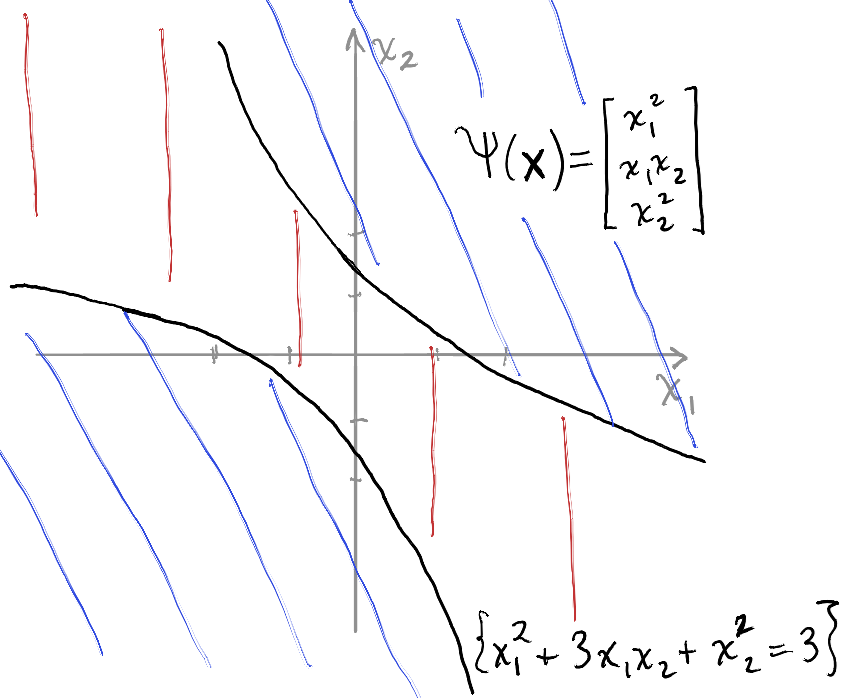
\includegraphics[height=0.35\textheight]{../../Images/kernel-figure.png}
        \end{wrapfigure}

    \textbf{Example.} Define $\psi:\mathbb R^2 \to \mathbb R^3$ so that, for \mbox{$\x=(x_1,x_2)$} we have 
    \vspace{-6pt}
    \[\psi(\x) = \begin{bmatrix}x_1^2 \\ x_1x_2 \\ x_2^2\end{bmatrix}.\]
    \vspace{-6pt}
    
    \pause
    Letting $\textbf{w} = \begin{bmatrix}1 \\ 3\\ 1\end{bmatrix}$ and $b = -3$, the set of points $\x\in\mathbb R^2$ such that $\textbf{w}\cdot\psi(\x) + b = 0$ is union of two curves depicted to the right.
    \end{minipage}
    \pause

    \medskip
    The set of $\x\in\mathbb R^2$ that this model would label positively are those such that $\textbf{w}\cdot\psi(\x) + b > 0$, shaded in blue. (A hyperplane in $\mathbb R^3$ separates images, under $\psi$, of positively and negatively labeled points.)
\end{frame}

%%%%
\begin{frame}
    \frametitle{SVMs with Non-linear Decision Boundaries}
    
    \medskip
    \begin{minipage}{\textwidth}
        \begin{wrapfigure}{r}{0.3\textwidth}
            \centering
            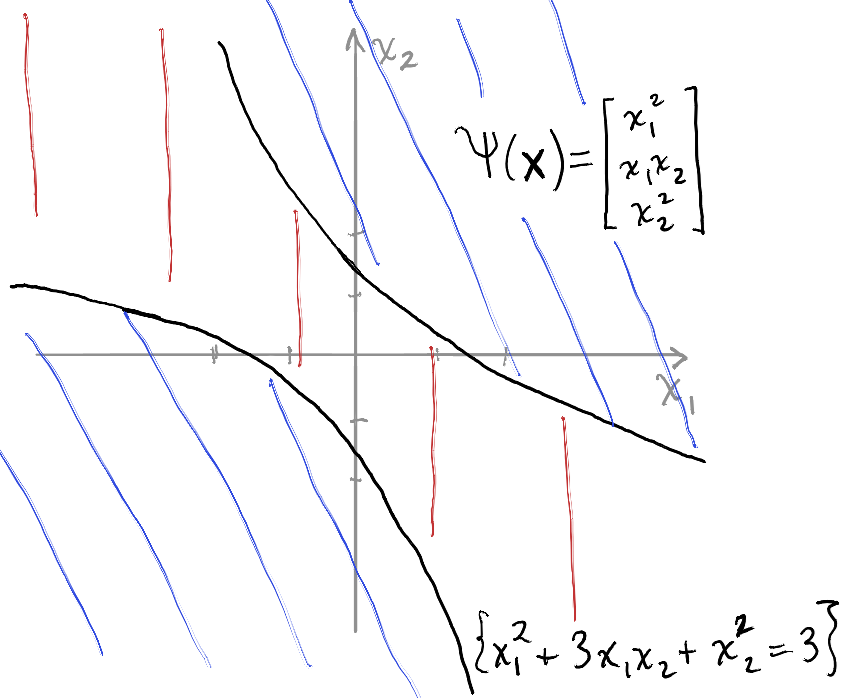
\includegraphics[height=0.35\textheight]{../../Images/kernel-figure.png}
        \end{wrapfigure}

    \textbf{Example (cont'd).} We have 
    \[\psi(\x) = \begin{bmatrix}x_1^2 \\ x_1x_2 \\ x_2^2\end{bmatrix}\]
    
    \vspace{-6pt}
    and $\textbf{w} = (w_1, w_2, w_3)$. Say that the data is modeled well by this \textit{type} of decision boundary (maybe not perfectly separated though).
    
    \pause
    Then solving the minimization problem, over $\textbf{w}\in\mathbb R^3$, $b\in\mathbb R$,
    \end{minipage}

    \medskip
        \[\min_{\textbf{w},b} \qquad\lambda|\textbf{w}|^2 + \frac{1}{n}\sum_{i=1}^n\max\{0, 1 - \ix y_i(\textbf{w}\cdot\psi(\x_i) + b)\}\]
    is a non-linear SVM (potentially with some points having a non-zero slack variable).
    
    \pause
    But, how can we do this? Especially if the map $\psi$ is not known beforehand?
\end{frame}

%%%%
\begin{frame}
    \frametitle{Lagrangian Dual Problem}
    Recall (from earlier SVM lecture), the Lagrange multiplier method leads to a ``dual'' maximization problem that is an equivalent one:\footnote{This is the version without slack variables. There is one with slack variables.}

    \[\max_{\emph{\alpha}} \sum_{i=1}^n\alpha_i - \frac12\sum_{i,j=1}^n\alpha_i\alpha_j\ix y_i\ix y_j (\x_i\cdot\x_j).\]

    \pause
    Note that this does not require knowing the actual points $\x_i\in\mathbb R^d$, only the dot products between pairs $\x_i$ and $\x_j$. It also does not require that we determine $(\textbf{w},b)$, but the multipliers $\alpha_1,\ldots,\alpha_n$ instead. \footnote{The Lagrange multipliers then, in turn, determine both $\textbf{w}$ and $b$.}

    \pause
    \medskip
    These observations are part of a more general phenomenon.
\end{frame}

%%%%
\begin{frame}
    \frametitle{Kernels - The Representer Theorem}
    Let $f:\mathbb R^n\to\mathbb R$ be an arbitrary function and let $R:\mathbb R_{\ge0}\to\mathbb R$ be an increasing\footnote{Really only need \textit{non-decreasing}: if $a_1<a_2$ then $R(a_1)\le R(a_2)$.} function. Further, say that we have a map $\psi:\mathbb R^d\to H$.\newline\pause  
    We consider the minimization problem 
        \[\min_{\omega} \qquad f\left(\langle\omega, \psi(\x_1)\rangle, \ldots, \langle\omega, \psi(\x_n)\rangle\right) + R(|\omega|). \qquad(\dag)\]
    \pause
    \vspace{-12pt}
    
    \begin{itemize}
        \item  Our SVM optimization is an instance of this with\footnote{Suppose last coordinate of $\psi(\x)$ to be 1 and $\omega = (\textbf{w}, b)$.} $f(a_1,\ldots,a_n) = \frac{1}{n}\sum \max\{0,1-\ix y_ia_i\}$ and $R(a) = \lambda a^2$.
    \end{itemize}
    \pause
    Often, $H = \mathbb R^D$ for some integer $D>0$. However, this theorem works more generally, $H$ being something called a \textit{Hilbert space}.
    \pause
    \begin{theorem}[Representer Theorem]
        There exists vector $\underline\alpha \in\mathbb R^n$ such that $\omega=\sum_{i=1}^n \alpha_i\psi(\x_i)$ is a minimizer of ($\dag$).
    \end{theorem}
    \pause
    \begin{proof}[Proof sketch] 
        {\small Given $\omega$ from theorem statement, if $\omega^*$ is minimizer, can write $\omega^* = \omega + \upsilon$ with $\upsilon$ orthogonal to $\psi(\x_i)$ for all $i$, which implies $|\omega|^2 \le |\omega^*|^2$.\pause\ This means $R(|\omega|)\le R(|\omega^*|)$; can check that $\ix y_i\langle\omega, \psi(\x_i)\rangle = \ix y_i\langle\omega^*, \psi(\x_i)\rangle$ for all $i$.\pause\ 
        Put together $\implies$ value of ($\dag$) on $\omega$ is not more than its value on $\omega^*$.}
    \end{proof}
\end{frame}

%%%%
\begin{frame}
    \frametitle{Kernel Trick}
    By the Representer Theorem, we can consider the optimal $\omega = \sum_{i=1}^n\alpha_i\psi(\x_i)$. Then we are able to rewrite the optimization problem ($\dag$).

    \begin{align*}
        \langle\omega, \psi(\x_j)\rangle &= \sum_{i=1}^n\alpha_i\langle\psi(\x_i), \psi(\x_j)\rangle \\
        |\omega|^2                      &= \langle\sum_{i=1}^n\alpha_i\psi(\x_i), \sum_{i=1}^n\alpha_i\psi(\x_i)\rangle = \sum_{i,j = 1}^n \alpha_i\alpha_j\langle\psi(\x_i), \psi(\x_j)\rangle.
    \end{align*}
    We put these expressions into $f$ and $R$ in ($\dag$); they only depend on $\alpha_1,\ldots, \alpha_n$ and the dot products\footnote{\textit{Inner products}, more generally.} between $\psi(\x_i)$ and $\psi(\x_j)$. 

    \pause
    A ``trick'': don't figure out $\psi$, but decide on a function $K(\x, \x')$ that will determine the dot products $\langle\psi(\x), \psi(\x')\rangle$.\pause\ Often the dimension $D$ used by $\psi$ needs to be fairly large and dot products in high dimension can be computationally expensive. However, if we choose $K$ and get the \textbf{Gram matrix}, with $(i,j)$ entry $K(\x_i, \x_j)$, such dot products not needed; optimize the parameters $\alpha_i$ only.
\end{frame}

%%%%
\begin{frame}
    \frametitle{Popular Kernel Functions}
    Two common choices for kernel function $K$ are listed below. In general, the corresponding Gram matrix should be symmetric and \textit{positive semi-definite}.

    \pause
    \begin{enumerate}
        \item \textbf{Polynomial kernels.} For constants $r\ge 0, \gamma>0$, and positive integer $d$, set 
            \[K(\x, \x') = (r + \gamma(\x\cdot\x'))^d.\]
        In the definition, $\x\cdot\x'$ is usually the standard dot product, but could be another inner product.
        \pause
        \item \textbf{Gaussian kernels.} For constant $\gamma > 0$, set 
            \[K(\x, \x') = e^{-\gamma|\x - \x'|^2}.\]
        These kernels are also called ``Radial Basis Function'' (RBF) kernels.
    \end{enumerate}

    \pause
    \begin{itemize}
        \item Think about a polynomial kernel with $r=\gamma=1$ and $d = 2$. Further, say that $\x$ and $\x'$ are in $\mathbb R^2$. Check that $\psi(\x) = (x_1^2, \sqrt{2}x_1x_2, x_2^2, \sqrt{2}x_1, \sqrt{2}x_2, 1)\in\mathbb R^6$ will give the equation 
            \[K(\x, \x') = \psi(\x)\cdot\psi(\x').\]
    \end{itemize}

\end{frame}



%%%%
\begin{frame}[fragile]
    \frametitle{SGD Procedure for SVM with Kernels (and slack variables)}
    Here is the SGD procedure with a kernel (using the Gram matrix $[K(\x_i, \x_j)]$).

    \pause
    The algorithm uses gradient descent to iteratively find $\alpha_1^{(t)},\ldots,\alpha_n^{(t)}$ at step $t$. During it, scalars $\beta_1^{(t)},\ldots,\beta_n^{(t)}$ are used. Writing \lstinline[language=Pseudo,basicstyle=\ttfamily]{beta[i][t]} for $\beta_i^{(t)}$ and \lstinline[language=Pseudo,basicstyle=\ttfamily]{psi} for $\psi$, the relation to our previous SGD algorithm is \lstinline[language=Pseudo,basicstyle=\ttfamily]{theta[t] = sum( beta[i][t]*psi(X[i]), i=1,...,n )}.
\pause

\begin{pseudo}
## lambda: the coeff of regularization; T: the number of iterations
## K: n by n Gram matrix
input: K, y, lambda, T
beta[i][1] = initial zero for i from 1,...,n
for (t == 1,...,T){
    alpha[i][t] = beta[i][t]/(2*lambda*t)  # for i from i,...,n
    Choose j uniformly at random from 1,...,n
    beta[i][t+1] = beta[i][t] # for i not equal j
    if (y[j]*sum( alpha[i][t]*K[i,j], i from 1,...,n ) < 1)
        beta[j][t+1] = beta[j][t] + y[j]
    else 
        beta[j][t+1] = beta[j][t]
}
return average (alpha[i][1], ..., alpha[i][T]) # for i from 1,...,n
\end{pseudo}

\pause
Note: The vectors $W^{(t)}$ of previous algorithm are $\sum_{i=1}^n\alpha_i^{(t)}\psi(\x_i)$. But, writing $\overline{W}$ for average of the $W^{(t)}$, to get prediction on unseen $\x\in\mathbb R^d$ we just need 
    
    \vspace{-7pt}
    {\small
    \[\langle\overline{W}, \psi(\x)\rangle = \sum_{i}\overline{\alpha}_i K(\x_i, \x).\]
    }
\end{frame}
\end{document}